	\documentclass[10pt,oneside]{CBFT_book}
	% Algunos paquetes
	\usepackage{amssymb}
	\usepackage{amsmath}
	\usepackage{graphicx}
% 	\usepackage{libertine}
% 	\usepackage[bold-style=TeX]{unicode-math}
	\usepackage{lipsum}

	\usepackage{natbib}
	\setcitestyle{square}

	\usepackage{polyglossia}
	\setdefaultlanguage{spanish}
	



	\usepackage{CBFT.estilo} % Cargo la hoja de estilo

	% Tipografías
	% \setromanfont[Mapping=tex-text]{Linux Libertine O}
	% \setsansfont[Mapping=tex-text]{DejaVu Sans}
	% \setmonofont[Mapping=tex-text]{DejaVu Sans Mono}

	%===================================================================
	%	DOCUMENTO PROPIAMENTE DICHO
	%===================================================================

\begin{document}

% =================================================================================================
\chapter{Dinámica cuántica}
% =================================================================================================

Queremos ver la evolución temporal de los kets. Para ello utilizaremos cierta convención.
Un ket dependerá del tiempo lo cual se indicará con 
\[
	\Ket{\alpha,t_0,t},
\]
notación que refiere al estado $\alpha$ que partió en $t_0$ al tiempo $t$. 
Luego $\Ket{\alpha,t=t_0} \equiv \Ket{\a}$.
Pictóricamente
\[
	\Ket{\alpha,t_0} \underbrace{\longrightarrow}_{\text{evoluciona}} \Ket{\alpha,t_0,t}
\]

Emplearemos para ello un operador de evolución temporal $U_{(t,t_0)}$ al cual le pediremos
que realice la evolución según
\[
	\Ket{\alpha,t_0,t} = U \Ket{\alpha,t_0}
\]
Entonces, un elemento de matriz $\Braket{b|U_{(t,t_0)}|a}$ implica la probabilidad (amplitud)
de que se tenga componente de $b$ en el tiempo $t$ del sistema que estamos considerando.
El operador de evolución tendrá las propiedades

\begin{itemize}
 \item Unitariedad
 \[
	\Braket{ \alpha,t_0,t| \alpha,t_0,t} = 1 \qquad \forall t
 \]
 \[
	\Braket{ \alpha,t_0| U^\dagger U| \alpha,t_0} = 1 \quad \Rightarrow \quad 
	U^\dagger U = U U^\dagger = \mathbb{1}
 \]
 para conservación de la probabilidad. Tiene que ser unitario.
 \item Linealidad
 \[
	U(t_2,t_0) = U(t_2,t_1) U(t_1,t_0) \qquad t_2>t_1>t_0
 \]
 \item Límite a $\mathbb{1}$ (identidad)
 \[
	U_{(t,t_0)} \to \mathbb{1} \quad \text{si} \quad t\to t_0
 \]
 o bien 
 \[
	U_{(t_0+dt,t_0)} \to \mathbb{1} \quad \text{si} \quad dt\to 0
 \]
\end{itemize}

Se propone entonces (infinitesimalmente) un 
\[
	U_{(t+dt,t)} = \mathbb{1} - i \: \Omega \: dt 
\]
con $\Omega$ hermítico. Comparando con clásica vemos que $H$ origina la evolución temporal, entonces
identificamos $\Omega$ con $H$, del modo $\Omega = H/\hbar$ así que 
\[
	U_{(t+dt,t)} = \mathbb{1} - \frac{i}{\hbar} H dt .
\]

De esta forma 
\[
	U_{(t+dt,t_0)} =  U_{(t+dt,t)} U_{(t,t_0)}  = 
	\left( \mathbb{1} - \frac{i}{\hbar} H dt \right) U_{(t,t_0)}
\]
\[
	\dpar{U}{t} = \lim_{dt\to 0} \frac{ U_{(t+dt,t_0)} - U_{(t,t_0)} }{dt} = 
	- \frac{i}{\hbar}H U_{(t,t_0)}
\]
y entonces 
\[
	i\hbar\dpar{U}{t} = HU
\]
que es la ecuación para $U_{(t,t_0)}$.
No podemos utilizar los métodos que usamos anteriormente porque en
$U = N \euler^{i \int dt' \:H(t)/\hbar }$ [depende del tiempo?].
Supongmos que es $ H \sim \vb S \cdot \vb r (\theta)$, se tiene en
$t=0$ es $\vb r(t) = \zver$ y en $t = 5 \text{ seg. } $ es $\vb r(t) = \yver$.
Tenemos
\[
	i\hbar\dpar{}{t} U_{(t,t_0)} \Ket{\alpha,t_0} = H U_{(t,t_0)} \Ket{\alpha,t_0},
\]
que nos conduce a la ecuación de Schrödinger para kets
\[
	i\hbar\dpar{}{t} \Ket{\alpha,t_0,t} = H \Ket{\alpha,t_0,t}
\]
donde el inconveniente es que $H=H(t)$.

El concepto se ilustra en la figura siguiente
\begin{figure}[htb]
	\begin{center}
	\includegraphics[width=0.3\textwidth]{images/teo2_5.pdf}	 
	\end{center}
	\caption{}
\end{figure} 

% % =================================================================================================
% \section{Dinámica cuántica}
% % =================================================================================================

\section{Casos sencillos de solución de $U(t,t_o)$}

\begin{itemize}
 \item Supongamos $ H \neq H(t)$, entonces
 \[
	U( t, t_0) = \euler^{-i/\hbar H (t-t_0)} 
 \]
 \item Sea $ H = H(t)$, entonces
 \[
	U( t, t_0) = \euler^{-i/\hbar \int_{t_0}^t H(t')dt'} 
 \]
 y la integral puede hacerse una vez conocida la expresión de $H(t)$.
 \item Sea $ H = H(t)$ con $[H(t_1),H(t_2)] \neq 0$ entonces
 \begin{multline*}
	U( t, t_0) =  1 + \sum_{n=1}^{\infty} \left( \frac{-i}{\hbar}\right)^n 
		\int_{t_0}^t dt_1 \int_{t_0}^{t_1} dt_2 \int_{t_0}^{t_2} dt_3 ... \times \\
			\int_{t_0}^{t_{n-1}} dt_n H(t_1) H(t_2) ... H(t_n)    
 \end{multline*}
%  \[
% 	U( t, t_0) =  1 + \sum_{n=1}^{\infty} \left( \frac{-i}{\hbar}\right)^n 
% 		\int_{t_0}^t dt_1 \int_{t_0}^{t_1} dt_2 \int_{t_0}^{t_2} dt_3 ... \int_{t_0}^{t_{n-1}} dt_n 
% 			H(t_1) H(t_2) ... H(t_n)  
%  \]
y esta es la serie de Dyson (del físico Freeman Dyson().)
Esta es la solución formal general para el caso 3. 
\end{itemize}

El problema que suscita es debido a que si $H$ a diferentes tiempos no conmuta
no podemos poner la exponencial en serie de potencias. 
En realidad $\exp({\square})$ tiene sentido sólo si la serie 
\[
	\sum_{n=0}^{\infty}  \frac{1}{n!}\square^n
\]
tiene sentido; es decir, si no surgen ambigüedades al tomar la potencia $n$-ésima
del operador $\square$.
\notamargen{El operador $\square$ no se deja poner sombreros, 
quiere andar con la cabeza descubierta}

Para el caso 1 (pensamos una especie de serie de Taylor, que es un modo general
de encarar este tipo de problemas de cosas no bien definidas) es simplemente 
\[
	\euler{-i\frac{H}{\hbar}(t-t_0)} = 1 - i\frac{H}{\hbar}(t - t_0) + 
	\frac{(-i)^2}{2}\left( \frac{H \Delta t }{\hbar} \right)^2 + ... +
	\frac{(-i)^n}{n!} \Frac{H\Delta t}{\hbar}^n,
\]
y por otra parte
\[
	i \hbar \dpar{}{t}U(t,t_0) = H - i \frac{H^2}{\hbar^2} \Delta t + ...
\]
y término a término coinciden; entonces probamos que la solución vale.

Para el caso 2, donde los hamiltonianos a diferentes tiempos conmutan entre
sí, es decir $ [ H(t_1), H(t_2) ] = 0 $ la solución es
\[
	U(t,t_0) = \euler^{ i/\hbar \int_{t_0}^t \: H(t') \: dt' }
\]

Esto no es una boludez. Al desarrollar Taylor la exponencial surge un problema

Si no conmutan los operadores no sé cómo armar el cuadrado.
\[
	A^2 = A(t)A(t'') \; \text{ o bien } \: A^2 = A(t'')A(t)
\]
\[
	\left( \int H(t') dt' \right)\left( \int H(t'') dt'' \right) \neq 
	\left( \int H(t'') dt'' \int H(t') dt' \right)
\]
puesto que al operar es 
\[
	\int dt' dt'' H(t')H(t'') \neq \int dt' dt'' H(t'') H(t') 
\]
pues $[H(t'),H(t'')]\neq 0$.
En el caso 2 $(\int_{t_0}^t H(t')dt' )^n$ no tiene problemas puesto que está 
provista la conmutatividad.

\subsection{Soluciones útiles}

La solucion que sirve es
\[
	\Ket{\a,t_0,t} = U(t,t_0)\Ket{\a}
\]
La idea es escribir el $\Ket{\a}$ del sistema y hallar un operador que conmute
con el hamiltoniano y en cuya base escribo $\Ket{\a}$,
\[
	\Ket{\a} = \sum C_{a'} \Ket{a'}
	\qquad \qquad 
	H \Ket{\a} = \sum E_{a'} C_{a'} \Ket{a'}
\]
y trabajaremos con una solución útil ahora.

Primeramente conseguimos un $\hat{A}$ tal que $[ A, H ]=0$ y entonces (estoy 
considerando $ H \neq H(t)$ )
\[
	\Ket{\alpha} = \sum_{a'} \Ket{a'}\Braket{\alpha'|\alpha},
\]
luego 
\[
	U(t,t_0)\Ket{\alpha} = \sum_{a'} \euler^{-i\frac{\hat{H}}{\hbar}(t-t_0)}
	\: \Ket{a'}\Braket{\alpha'|\alpha}
\]
con $\hat{H}$ y $\hat{A}$ conmutan se tiene
\[
	\hat{H}\Ket{a'}=E_{a'}\Ket{a'} \qquad \hat{A}\Ket{a'}= a'\Ket{a'}
\]

Entonces operamos con el $H$ para 
\[
	U(t,t_0) = \sum_{a'} \euler^{-i\frac{E_{a'}}{\hbar}(t-t_0)}\Ket{a'}\Bra{a'}
\]
y así (quiero saber cómo trabaja en el tiempo $\Ket{\a}$), le aplico el operador
evolución
\[
	U(t,t_0)\Ket{\alpha} = \sum_{a'} 
	\euler^{-i\frac{E_{a'}}{\hbar}(t-t_0)}\Ket{a'}\Braket{a'|\alpha}
\]
\[
	\Ket{\alpha,t_0,t} = \sum_{a'} \Braket{a'|\alpha}
	\euler^{-i\frac{E_{a'}}{\hbar}(t-t_0)} \: \Ket{a'} =
	\sum_{a''} \sum_{a'} c_{a'} \euler^{-i\frac{E_{a'}}{\hbar}(t-t_0)} \: 
	\Ket{a''}\Braket{a''|a'}
\]
o bien
\[
	\Ket{\alpha,t_0,t} = \sum_{a'} 
	c_{a'} \euler^{-i\frac{E_{a'}}{\hbar}(t-t_0)} \: \Ket{a'},
\]
de manera que comparando con 
\[
	\Ket{\alpha,t_0} = \sum_{a'} \Braket{a'|\alpha} \Ket{a'}
\]
El coeficiente es el mismo pero le hemos sumado una fase 
$\exp(-iE_{a'}(t-t_0)/\hbar)$ que no es global.

\subsection{Evolución de valores de expectación}

Recordemos primeramente que los autoestados no evolucionan. Luego 
\[
	\Ket{\alpha} = \Ket{a'} 
	\qquad \to \qquad 
	\Ket{\alpha,t} = \Ket{a',t} =  
	\euler^{-i\frac{E_{a'}}{\hbar}(t-t_0)} \Ket{a'}
\]

La fase es global y no tiene sentido físico (no cambia el valor de expectación, por ejemplo)
Es considerar una autoestado [?]. La podemos descartar (setear igual a uno)
\[
	\Braket{a',t|B|a',t} = 
	\braket{a'|\euler^{i\frac{E_{a'}}{\hbar}(t-t_0)}B 
	\euler^{-i\frac{E_{a'}}{\hbar}(t-t_0)}|a'} = \braket{a'|B|a'}
\]

El valor de expectación de un operador respecto a un autoestado no varía.
Se simplifican las fases y en el valor de expectación no me entero de ellas.
Para un estado que no es necesariamente autoestado
\[
	\braket{\alpha,t|B|\alpha,t} =
	\braket{a''|\sum_{a''} \braket{a''|\alpha}^*\euler^{i\frac{E_{a'}}{\hbar}(t-t_0)} B 
	\sum_{a'} \braket{a'|\alpha} \euler^{-i\frac{E_{a'}}{\hbar}(t-t_0)}|a'}
\]
\[
	\braket{\alpha,t|B|\alpha,t} = \sum_{a',a''} C_{a''}^* C_{a'} 
	\euler^{i\frac{E_{a''}-E_{a'}}{\hbar}(t-t_0)} \braket{a''|  B |a'}
\]
donde $(E_{a''}-E_{a'})/\hbar$ es la llamada frecuencia de Bohr y vemos que la fase
global depende de los índices de las sumatorias; entonces habrá términos de interferencia.
\[
	C_{a''}^* = \braket{\alpha,t_0|a''} \qquad C_{a'} = \braket{a'| \alpha,t_0}  
\]

El valor de expectación de un operador respecto a un estado general tiene una fase no global 
que produce términos de interferencia.

Sólo en el caso en que $B$ conmute con $H$ ($B$ diagonal) se dará que la fase no interviene,
porque pierdo una sumatoria merced a una delta de Kronecker que aparece.

\subsection{Relaciones de conmutación}

\[
	[ A + B, C] = [A, C] + [B,C] 
\]
\[
	[A, B] = - [B,A]
\]
\[
	[A, B\cdot C] = B[A,C] +  [A,B]C
\]
\notamargen{Acá no es baca + caballo puesto que no conmutan.}
\[
	i\hbar[ A, B]_{\text{classic}} = [A, B]
\]
donde $[ , ]_{\text{classic}}$ es el corchete de Poisson.
Las relaciones de conmutación fundamentales son 
\[
	[x_i, x_j] = 0 \qquad [p_i, p_j]=0 \qquad [x_i,p_j] =i\hbar\delta_{ij}
\]
a las que podemos sumar
\[
	[x,f(p)] = i\hbar\dpar{f}{p} \qquad [p,G(x)] = i\hbar\dpar{G}{x} 
\]
\[
	[S_i,S_j] = i\hbar \varepsilon_{ijk}S_k
\]

\subsection{La ecuación de Schrödinger}

\[
	i\hbar\dpar{}{t}\Ket{\alpha,t_0,t} = H\Ket{\alpha,t_0,t} \text{con} 
	\qquad \hat{H} = \frac{\hat{p}^2}{2m} + V(\hat{x}) 
\]
Puedo meter un bra $\Bra{x'}$ que no depende del tiempo y entonces 
\[
	i\hbar\dpar{}{t}\braket{x'|\alpha,t_0,t} = \braket{x'|H|\alpha,t_0,t}
\]
\[
	i\hbar\dpar{}{t}\Psi_\alpha(x',t) = \braket{x'|\frac{p^2}{2m} + V(x)|\alpha,t_0,t}
\]
de manera que resulta la ecuación de Schrödinger
\[
	i\hbar\dpar{}{t}\Psi_\alpha(x',t) = -\frac{\hbar^2}{2m}\dpar[2]{}{x}\Psi_\alpha(x',t) + 
	V(x)\Psi_\alpha(x',t)
\]

\subsection{Representación de Heisenberg}

Los kets y los operadores no tienen sentido físico, pero sí los valores de expectación : toda física podrá modificar 
los primeros pero debe conservar los valores de expectación. Así tenemos dos representaciones posibles:

\begin{center}
\begin{tabular}{|l|l|}
\hline
Schrödinger & Heisenberg \\
\hline
& \\
$\Ket{\alpha} \to U\Ket{\alpha} \quad $ & $\Ket{\alpha} \to \Ket{\alpha} \quad $ \\
& \\
$A \to A \quad $ & $A \to U^\dagger AU \quad$ \\
& \\
$\Ket{a'} \to \Ket{a'} \quad $ & $\Ket{a'} \to U^\dagger \Ket{a'} \quad $ \\
& \\
\hline
\end{tabular}
\end{center}
Así vemos que en Schrödinger los kets evolucionan y los operadores permanecen fijos; al igual que los autoestados.
En cambio en Heisenberg los kets no evolucionan pero sí lo hacen los operadores y los autoestados.

Deben notars que:
\begin{enumerate}
 \item Los productos internos no cambian con el tiempo
 \[
	\braket{\beta|\alpha} = \braket{\beta|U^\dagger U|\alpha} 
 \]
 \item Los valores de expectacion son los mismos en ambos esquemas
 \[
	\braket{\alpha,t|A|\alpha,t} = \braket{\alpha,t|U^\dagger AU|\alpha,t} =
	\begin{cases}
	 \braket{A}^{(H)} \\
	 \braket{A}^{(S)}
	\end{cases}
 \]
 de lo cual se deduce que 
 \[
	\Braket{A}^{(S} = \Braket{A}^{(H} \qquad A(t)^H = U(t)^\dagger A^S U(t)
 \]
\end{enumerate}

El operador $\hat{A}$ en Schrödinger no depende explícitamente del tiempo. La idea es que le ``pegamos'' a los 
operadores la evolución temporal de los kets.
\[
	(\Bra{ \alpha, t_0 } U^\dagger) A^{(S)} (U \Ket{\alpha, t_0 }) = 
	\braket{ \alpha, t_0 | U^\dagger A^{(S)} US | \alpha, t_0 }
\]
pero a $t=t_0$ las representaciones coinciden,
\[
	\Ket{\alpha,t_0,t_0}^{(S)} = \Ket{\alpha}^{(H)}
\]

\subsubsection{La ecuación de Heisenberg}

\[
	A^H = U^\dagger A^S U \qquad \dpar{A^H}{t} = \dpar{U^\dagger}{t}A^S U + U^\dagger A^S \dpar{U}{t} +
	U^\dagger A^S \dpar{U}{t}
\]
\[
	i\hbar \dpar{U}{t} \Rightarrow  \dpar{U}{t} = \frac{1}{i\hbar}HU \; \text{;} \;
	\dpar{U^\dagger}{t} = \frac{1}{-i\hbar}U^\dagger H
\]
\[
	(HU)^\dagger = U^\dagger H^\dagger = U^\dagger H 
\]
\[
	\dpar{A^H}{t} = \frac{-1}{i\hbar} U^\dagger H A^S U + \underbrace{U^\dagger\dpar{A^S}{t} U}_{=0} +
	U^\dagger A^S \frac{1}{i\hbar} H U
\]
pues $A^S$ no depende explícitamente del tiempo
\[
	\dpar{A^H}{t} = -\frac{1}{i\hbar} \left( U^\dagger HUU^\dagger A^SU -U^\dagger A^S U U^\dagger 
	HU \right) =	\frac{1}{i\hbar}(-HA + AH)
\]
y llegamos a la ecuación de Heisenberg
\[
	\dpar{A^{(H)}}{t} = \frac{1}{i\hbar} [ A^{(H)}, H^{(H)}]
\]
si $A^{(H)}$ conmuta con el $H^{(H)}$, entonces $A^{(H)}$ es una cantidad conservada (una constante de movimiento).
En ese caso el operador no depende del tiempo y entonces $A^{(H)} = A^{(S)}$.

\subsubsection{Evolución de autoestados}

\[
	A^S \Ket{a'}^S = a' \Ket{a'}^S,
\]
aplico un $U^\dagger$ a ambos lados y entonces 
\[
	U^\dagger A^S UU^\dagger \Ket{a'}^S = a' U^\dagger \Ket{a'}^S
\]
los $a'$ no dependen de la representación porque tienen significado físico. Entonces los $\Ket{a'}$ evolucionan
\[
	A^H (U^\dagger\Ket{a'}^S) = a' (U^\dagger\Ket{a'}^S)
\]
\[
	\Ket{a',t}^H = U^\dagger \Ket{a'}^S \qquad \qquad \dpar{}{t}\left( \Ket{a',t}^H \right) = 
	\dpar{}{t} \left( U^\dagger \Ket{a'}^S \right)
\]
\[
	\dpar{}{t}\Ket{a',t}^H = -\frac{1}{i\hbar} U^\dagger \Ket{a'}^S =  -\frac{1}{i\hbar} H U^\dagger 
	\Ket{a'}^S
\]
puesto que recordemos, nota importante,
\[
	H^H = U^\dagger H^S U = U^\dagger U H^S = \mathbb{1}H^S = H^S
\]
entonces $H$ es el mismo en ambas puesto que $\hat{U} =\hat{U}(\hat{H})$ y $[U,H]=0$.

De esta forma los autoestados evolucionan al revés 
\[
	i\hbar \dpar{}{t} \Ket{a',t}^H = -H\Ket{a',t}^H
\]

Podemos ver de otro modo la equivalencia
\[
	A^H = U^\dagger \sum_{a'} A^S \Ket{a'}\Bra{a'}U = 
	\sum_{a'} a'U^\dagger \Ket{a'}\Bra{a'}U
\]
pero 
\[
	A^H = \sum_{a'} A^H \Ket{a',t}\Bra{a',t} \equiv \sum_{a'}
\]
\[
	A^H = \sum_{a'} a' \Ket{a',t}\Bra{a',t} \equiv \sum_{a'} a'(U^\dagger\Ket{a'})(\Bra{a'}U)
\]
\[
	\Ket{a',t} = U^\dagger\Ket{a'}^S
\]

\subsubsection{Coeficientes}

Los coeficientes en Schrödinger y en Heisenberg son 
\[
	C_{a'}^S(t) = ^S\braket{a'|\alpha,t_0,t}^S = ^S\Bra{a'}(U\Ket{\alpha,t_0}) \qquad 
	C_{a'}^H(t) = ^H\braket{a',t|\alpha,t_0}^H = (^S\Bra{a'}U)\Ket{\alpha,t_0}
\]
Entonces en Schrödinger es 
\[
	\Ket{\alpha,t_0,t} = \sum_{a'} \Ket{a'}\braket{a'|\alpha,t_0,t} = 
	\sum_{a'} \overbrace{\braket{a'|\alpha,t_0,t}}^{C_{a'}(t)}\Ket{a'}
\]
mientras que en Heisenberg es 
\[
	\Ket{\alpha,t_0} = \sum_{a'} \Ket{a',t}\braket{a',t|\alpha,t_0} = 
	\sum_{a'} \overbrace{\braket{a',t|\alpha,t_0}}^{C_{a'}(t)}\Ket{a',t}
\]

Los coeficientes en las expresiones son iguales como corresponde a todo magnitud que tiene sentido físico, pues 
$|c_a(t)|^2$ es la probabilidad.

\subsection{Teorema de Ehrenfest}

Para una partícula libre, donde $p(t)=p(0)$ es constante de movimiento,
\[
	x^{(H)} = x(0) + \frac{p(0)}{m}t
\]
y se tiene 
\[
	[x(t),x(0)] = -\frac{i\hbar}{m}t
\]
que es decir que es un operador que no conmuta a $t$ diferentes
\[
	H = \frac{p^2}{2m} + V(x)
\]
\[
	\dtot{P}{t} = \frac{1}{i\hbar}[p,H] = \frac{1}{i\hbar}[p,V(x)] = 
	\frac{1}{i\hbar}\left( -i\hbar\dpar{V}{x}\right),
\]
de modo que 
\[
	\dtot{P}{t} = -\dpar{V}{x} \qquad \longrightarrow \quad m \dtot[2]{x}{t} = -\dpar{V}{x} 
\]
\[
	p = m \dtot{x}{t} \qquad \dtot{p}{t} = m \dtot[2]{x}{t} 
\]
donde estamos usando 
\[
	\dpar{A^H}{t} = \frac{1}{i\hbar}[A^H,H]
\]

Es necesario remarcar que relaciones como $[x,p]=i\hbar$ son para operadores en la picture de Schrödinger, donde los 
operadores no cambian en el tiempo. Estamos en efecto haciendo $[x(0),p(0)]=i\hbar$
\[
	\Braket{\alpha,t_0|m \dtot[2]{x}{t}|\alpha,t_0} = - \Braket{\alpha,t_0|\dpar{V}{x}|\alpha,t_0}
\]
\[
	m\dpar[2]{}{t}\Braket{\alpha,t_0| x^H |\alpha,t_0} = -\Braket{\alpha,t_0|\dpar{V}{x}|\alpha,t_0}
\]
y entonces el teorema de Ehrenfest es 
\[
	m \dpar[2]{}{t} \Braket{x^{(s)}} = - \Braket{ \dpar{V^{(s)}}{x}}
\]
los valores de expectación son iguales en ambas representaciones.



% \begin{figure}[htb]
% 	\begin{center}
% 	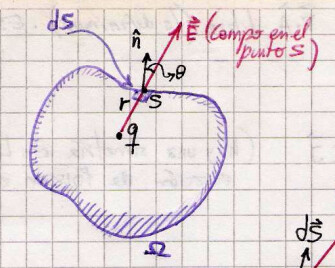
\includegraphics[width=0.35\textwidth]{images/fig_ft1_gauss.pdf}	 
% 	\end{center}
% 	\caption{}
% \end{figure} 




% \bibliographystyle{CBFT-apa-good}	% (uses file "apa-good.bst")
% \bibliography{CBFT.Referencias} % La base de datos bibliográfica

\end{document}
